\documentclass[11pt]{standalone}
\usepackage{pgf, tikz}
\usetikzlibrary{arrows, automata}
\begin{document}
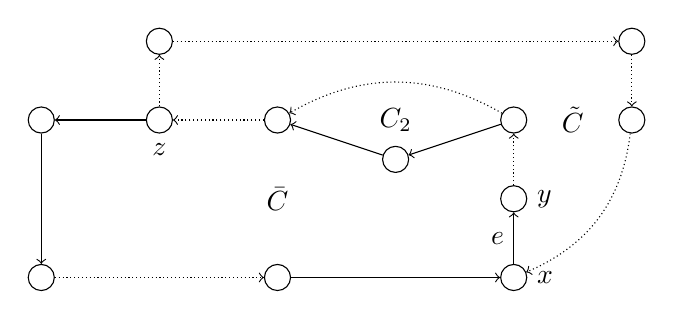
\begin{tikzpicture} [align=center]
\path (0,0) node[circle, draw] (v0) {}
	  (3,0) node[circle, draw] (v1) {}
	  (6,0) node[label={right:$x$},circle, draw] (v2) {}
	  (6,1) node[label={right:$y$},circle, draw] (v3) {}
	  (6,2) node[circle, draw] (v4) {}
	  (4.5,1.5) node[circle, draw] (v5) {}
	  (3,2) node[circle, draw] (v6) {}
	  (1.5,2) node[label={below:$z$},circle, draw] (v7) {}
	  (0,2) node[circle, draw] (v8) {}
	  
	  (7.5,2) node[circle, draw] (v9) {}
	  (7.5,3) node[circle, draw] (v10) {}
	  (1.5,3) node[circle, draw] (v11) {}
	  
(3,1) node (c1) {$\bar{C}$}
(4.5,2) node (c2) {$C_2$}
(6.75,2) node (c3) {$\tilde{C}$};
	  
\draw[densely dotted, ->] (v0) to (v1);
\draw[->] (v1) to (v2);
\draw[->] (v2) to node[left] {$e$} (v3);
\draw[densely dotted, ->] (v3) to (v4);
\draw[->] (v4) to (v5);
\draw[->] (v5) to (v6);
\draw[densely dotted, ->] (v6) to (v7);
\draw[->] (v7) to (v8);
\draw[->] (v8) to (v0);

\draw[densely dotted, ->] (v4) to [bend right] (v6);
\draw[densely dotted, ->] (v7) to (v11);
\draw[densely dotted, ->] (v11) to (v10);
\draw[densely dotted, ->] (v10) to (v9);
\draw[densely dotted, ->] (v9) to [bend left] (v2);
	  
\end{tikzpicture}
\end{document}